\begin{figure}[t]
  \centering
  \begin{tikzpicture}
    \node[inner sep=4pt, draw=gray!65, line width=0.5pt,
          fill=white,
          path picture={%
            \draw[step=0.25cm, gray!12, line width=0.15pt]
              (path picture bounding box.south west)
              grid (path picture bounding box.north east);
          }] {%
      \begin{minipage}{0.88\columnwidth}
        \centering
        \begin{subfigure}[t]{0.32\linewidth}
          \centering
          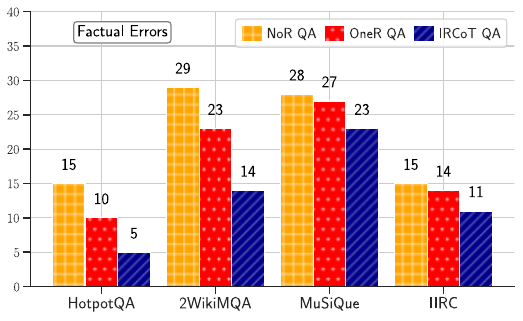
\includegraphics[width=\linewidth]{figures/fig_042_original.png}
          \caption{Original}
        \end{subfigure}\hfill
        \begin{subfigure}[t]{0.32\linewidth}
          \centering
          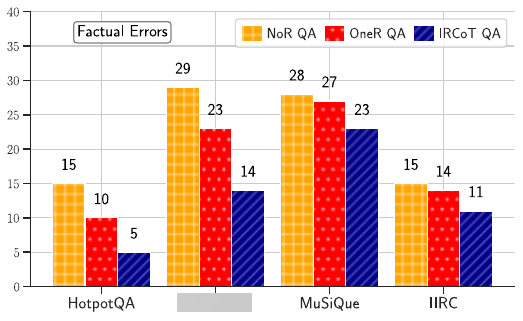
\includegraphics[width=\linewidth]{figures/fig_042_admittance.png}
          \caption{Admittance blur}
        \end{subfigure}\hfill
        \begin{subfigure}[t]{0.32\linewidth}
          \centering
          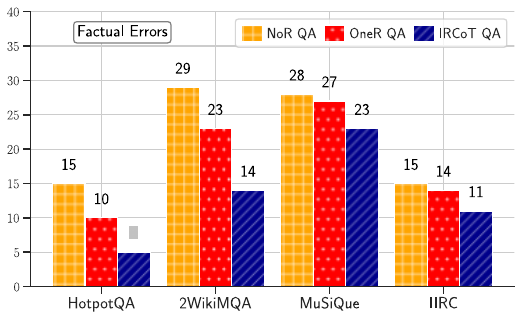
\includegraphics[width=\linewidth]{figures/fig_042_inductance.png}
          \caption{Inductance blur}
        \end{subfigure}
      \end{minipage}%
    };
  \end{tikzpicture}
  \caption{Selective blur for A-R-I evaluation. \textbf{(a)}~Original figure. \textbf{(b)}~Admittance blur: the dataset label ``2WikiMQA'' is obscured and cannot be recovered from context. \textbf{(c)}~Inductance blur: a value annotation is obscured but remains inferable from the y-axis scale.}
  \label{fig:blur-triptych}
\end{figure}
